\documentclass[12pt]{article}
\usepackage{amsmath,amsfonts, epsfig}
\usepackage{booktabs} % for better table formatting
\usepackage{array}
\usepackage{multirow}
\usepackage{graphicx}
\usepackage{fancyhdr}
\usepackage{bm}
\pagestyle{fancy}
\lfoot{\texttt{ematm0067.github.io}}
\lhead{Introduction to AI - 04.2\_HAC - Conor}
\rhead{\thepage}
\cfoot{}

\usepackage{tikz}
\usetikzlibrary{positioning}

\usetikzlibrary{shapes.misc}


\usepackage{ifthen,calc}
\newboolean{nopics}
\setboolean{nopics}{false}


\begin{document}

\section*{Hierarchical agglomerative clustering}

Lots of data sets have structure at different scales, to a certain
extent we saw that with the Hawk dataset, there were two properties
that separated the data into clusters in the wing length and weight
space, one was species and the other was probably sex. The difficulty
in clustering the data arose from the overlapping of the two scales,
the difference between the two genders for the RT hawks matched the
species difference between the SS and CH hawks. Of course, in the case
of $k$-means clustering we dealt with the number of clusters, rather
than the scale of clusteriness, though the two are roughly
reciprocally related. Here though we will talk about scale and the
idea is that it might be hard to see what scale is appropriate for
examining clusters in a dataset, or we might be interested in
different scales, or different sizes of cluster at the same time.

This is where hierarchical cagglomerative clustering, or HAC, is
useful; it is a map of the entire clustering structure of the data, up
to the usual sort of caveats that it only reliably finds simple,
glob-shaped, structures. The idea is to start with all the data and
identify the two closest data points. These are then joined together
to form a cluster, once they are clustered they are treated as a
single data point. Of course that means working out the distance of
this new point, representing the small cluster, and all the other data
points, there are various ways to do that and we will discuss that,
the most straight forward is the average, so if $\mathbf{a}$ and
$\mathbf{b}$ are the two points added to make the cluster
$\{\mathbf{a},\mathbf{b}\}$ then the distance from this to a point
$\mathbf{c}$ is
\begin{equation}
  d(\mathbf{c},\{\mathbf{a},\mathbf{b}\})=\frac{1}{2}[d(\mathbf{c},\mathbf{a}+d(\mathbf{c},\mathbf{b})]
\end{equation}
Now we just keep going, at every step merging the two closest points
to make a cluster, or a bigger cluster, and then recalculating
distances and iterating again until at the very end there is one big
cluster with all the points in.

\subsection*{An example - the DKB data}

This is easiest to see from an example; we will look at the DKB data
set \cite{DyanKruskalBlack1992}, this gives a set of distances between different languages. We
will describe how these distances are calculated soon but first of,
this is a very satifying sort of example because languages clearly
have a multi-scale clustering structure, even if people attempt to
create clusters by calling one set of languages `English' and another
`Norwegian', it is clear this is entirely artificial; as an
Irish-English speaker the language I speak is clearly different from
other Englishes spoken in Bath where I live and in my house my
children use a young peoples English which is different from mine,
even some very basic words are different, I eat my dinner, my daugher
scrans hers. In the case of Norwegian, there are two very different
sorts of Norwegian, Bokm\o{a}l and Nynorsk, both of which are called
Norwegian even if are not much less different from each other as they
from other nearby language like Danish. At a larger scale, Norwegian,
like English, is a Germanic language, French a Romance language and
Irish, the language spoken in Ireland along with Irish-English is a
Celtic langauge and all these clusters can be further grouped in
Indo-European languages.

The other nice thing about doing HAC on languages is that you might
expect that languages diverge at a roughly fixed rate so the
clustering describes their evolutionary history.

The DKB dataset uses a set of standard words, called a \textsl{Swadesh
  set} after a linguist called Morris Swadesh, which contains words
for basic actions, like eating and sleeping, and common objects like
the obvious body parts and things like fire and water. The most common
equivalents of these words are found for 84 different Indo-European
languages. Next, for any pair of these words, for example,
\textsl{sleep} and \textsl{schlafen}, words with the same meaning in
English and German, the word origins are studied to see if they have
the same etymology. In the case of \textsl{sleep} and
\textsl{schlafen} the answer is yes, they both come from the same
Proto-Germanic word, they are \textsl{cognate}. Ihe Irish for sleep,
however, is \textsl{coladh} which is not related to the German or
English word; French, \textsl{dormir}, Italian, \textsl{dormire},
Spanish, \textsl{dormir}, Portuguese, \textsl{dormir} and Romanian,
\textsl{dormi} all have cognate words with the same Latin origin. The
distance between two languages is then defined as the number of
non-cognate pairs divided by the total number of pairs. In the DKB
dataset a 200 word Swadesh list is used, so generally the number of
pairs of words for each pair of languages is 200, though, in a few
cases the translated list was incomplete.

Anyway, the upshot is that the DKB dataset is a matrix of distances
between 84 languages. We can apply HAC to this using a standard
library; we can also plot the resulting \textsl{dendrogram}, the
clustering libraries tend to have nice graphing commands that show a
tree of the clusters merging in a way that matches the separation of
the points being merged. Again, this is more obvious from a graph, the
HAC for all 84 languages is shown in Fig.~\ref{fig:big_HAC}. This
dendrogram has been coloured to show some of the clusters, for this the
number of clusters was specified.

It is clear that HAC has succeeded in discovering something
interesting in the data, the coloured groups largely represent
recognizable language families. The olive green are mostly Slavic
languages, though Latvian and Lithuanian aren't Slavic, the grey are
Germanic, the magenta are Romance, brown is Indo-Aryan, purple is
Iranian, red is just Albanian and green is Celtic; the orange is
confusing since Greek and Armenian are not normally thought of as
closely related languages. At a lower level, Dutch, Flemish and
Afrikaans are close to each other, for example, as are the two
dialects of Irish.

Clearly this graph doesn't match evolution, the Celtic languages, for
example, did not diverge from Greek more recently than they diverged
from Latin. Indeed, the idea that language evolution is a tree is
wrong, languages have multiple influences, they are not just the
isolated descendants of a parent language; indeed, they may have more
than one parent. The creoles are a particularly important example of
that and the HAC approach does not work well with creoles. The
location of Haitian Creole doesn't put it any closer to French than to
the other Romance languages, the complex history of Haitian Creole is
beyond anything that this approach can detect. The other creole,
Sranan Tongo, called here Taki-Taki, is placed in a similar way
relative to its closest Indo-European languages.


\begin{figure}[hp]
\begin{center}  
  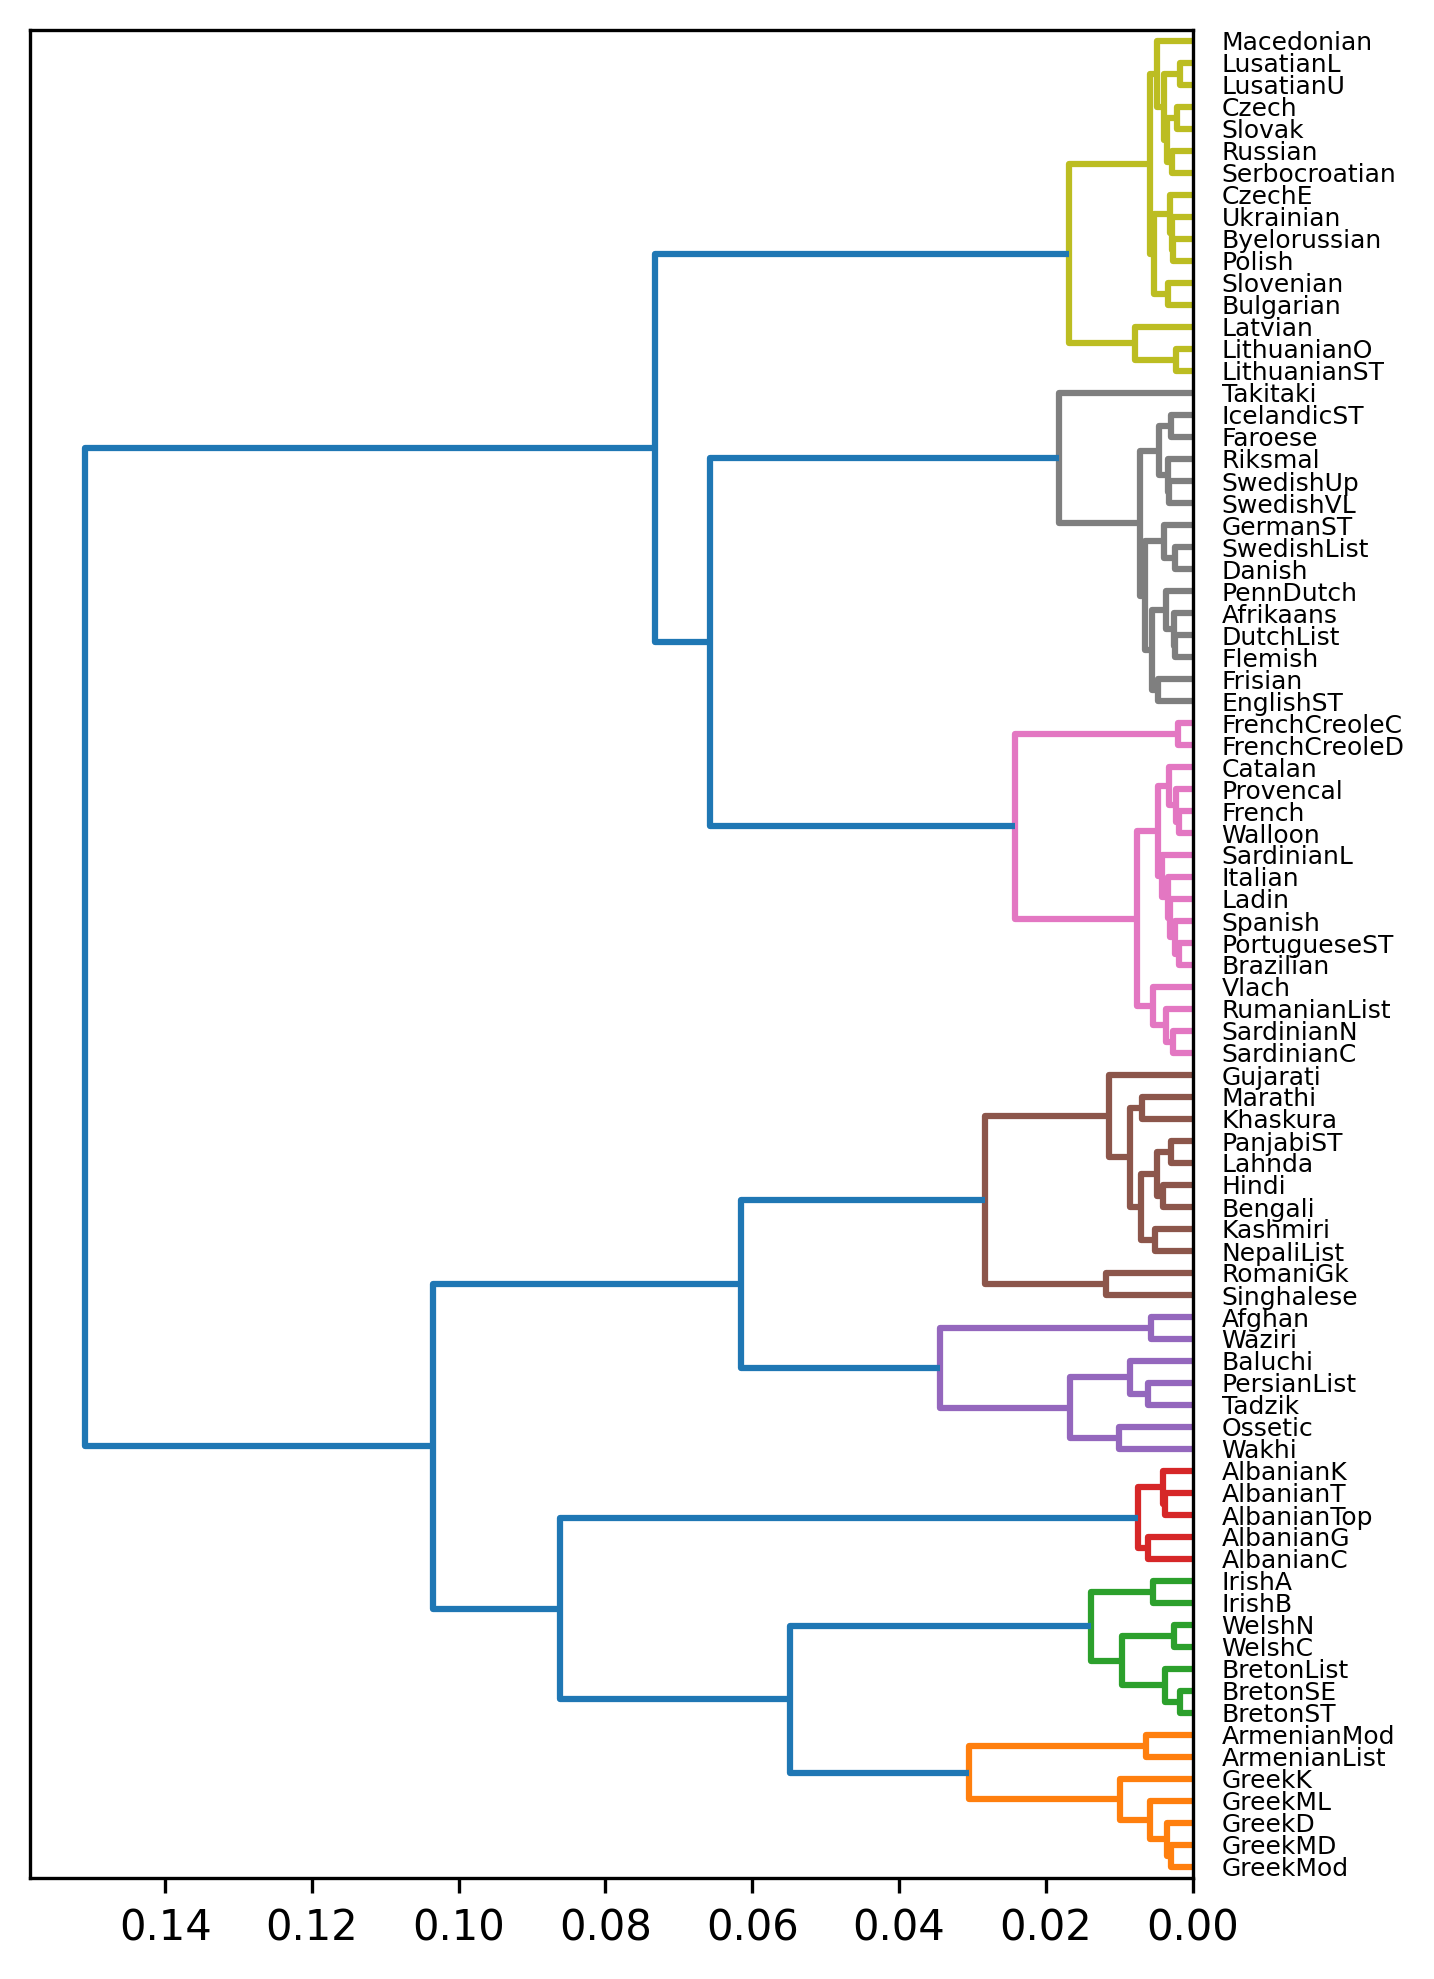
\includegraphics{dendrogram_big.png}
\end{center}
\caption{A dendrogram for the DKB language data; the languages are
  merged into larger and larger clusters, with the merge points placed
  on the $x$-axis at a distance between the two points or clusters when they merge.\label{fig:big_HAC}}
\end{figure}

\subsection*{Distances}

Above we glossed over the question of how we work out new distances as
we merge clusters; the example was given of using the average, so the
distance between any two clusters is the average distance between each
pair of one point from one cluster and one point from the other:
\begin{equation}
  d(C_1,C_2) = \frac{1}{|C_1||C_2|}\sum_{x\in C_1}\sum_{y\in C_2}d(x,y)
\end{equation}
This is one way to proceed, another would be to pick the smallest distance:
\begin{equation}
d(C_1,C_2)=\text{minimum}[d(x,y)|x\in C_1,y\in C_2]
\end{equation}
This is known as \textsl{single linkage}, if the largest distance is used
\begin{equation}
d(C_1,C_2)=\text{maximum}[d(x,y)|x\in C_1,y\in C_2]
\end{equation}
this is called \textsl{complete linkage}. 

The most common approach, \textsl{Ward linkage}, the one used for the
figure, is more complicated than the merge-the-nearest-clusters
strategy we have discussed so far. It is sometimes phrased in a
different way as an attempt to minimize an objective function,
typically the variance of the clusters as they are formed. This means
that it assesses clusters by calculating the \textsl{within-cluster variance}:
\begin{equation}
  V(C)=\frac{2}{|C|(|C|-1)}\sum{y\not=x,y\in C}\sum_{x\in C} d(x,y)^2
\end{equation}
of the potential new clusters; this allows the increase in
within-cluster variance to be calculated: if $C=C_1\cup C_2$ the increase in variance is
\begin{equation}
  \Delta V=V(C)-V(C_1)-V(C_2)
\end{equation}
and the merger with the smallest $\Delta V$ is the one that is
performed.

\begin{thebibliography}{9}

\bibitem{DyenKruskalBlack1992}
Dyen, I., Kruskal, J. B., \& Black, P. (1992). An Indoeuropean classification: A lexicostatistical experiment. \textit{Transactions of the American Philosophical Society}, \textit{82}(5), iii--132.

\end{thebibliography}

\end{document}

